\section{System's Perspective}

\subsection{Architecture and Design}
The ITU-MiniTwit system follows a modular client-server architecture designed to simulate the behavior of a micro-blogging platform. The system is composed of three main components:

\begin{itemize}
  \item \textbf{Web Application:} The frontend interface allows users to register, log in, follow other users, and post messages. This component communicates exclusively with the backend API.
  
  \item \textbf{API Server:} The API layer, serves as the core backend of the application. It handles user authentication, message posting, follower relationships, and provides all necessary endpoints for both the frontend and simulator.
  
  \item \textbf{Database:} A PostgreSQL database stores persistent data including user accounts, messages, and social connections. The API server interacts with the database through an ORM instead of direct SQL queries.
\end{itemize}

This separation of concerns enables a clean and maintainable architecture. It also supports scalability and facilitates the inclusion of automated testing and simulation tools. The API-first design ensures that the system can be extended or consumed by other services independently of the frontend implementation.

A simulation module is also integrated, which emulates realistic user behavior and interacts with the API to test the system's functionality and performance under load. Figure \ref{fig:simple-architecture} shows high level module view of how the systems interact. Simulator and Web application access API while API does all read/writes on the DB. 

\begin{figure}[H]
  \centering
  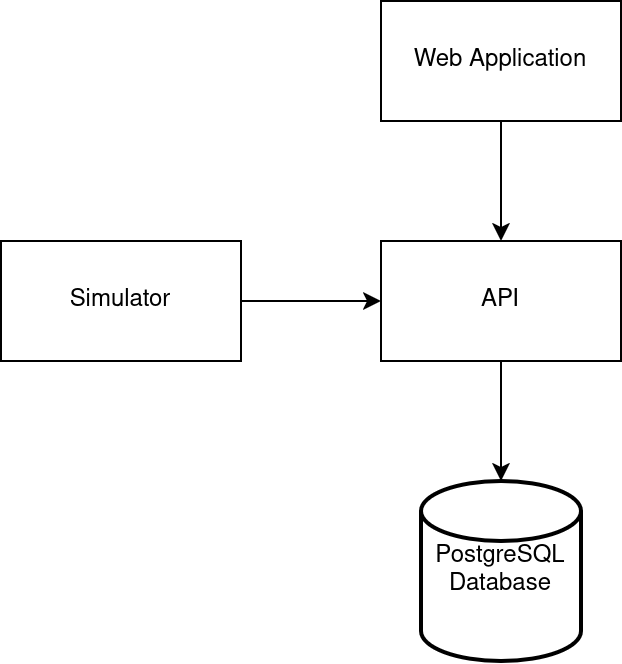
\includegraphics[width=0.4\textwidth]{report/images/simple-arch.png}
  \caption{High-level architecture of the system}
  \label{fig:simple-architecture}
\end{figure}

In our system, we also integrated monitoring tools. While details of which is explained in Section \ref{sec:monitoring} in detail, Figure \ref{fig:monitoring-arch} shows how it is integrated into our system. 

\begin{figure}[H]
  \centering
  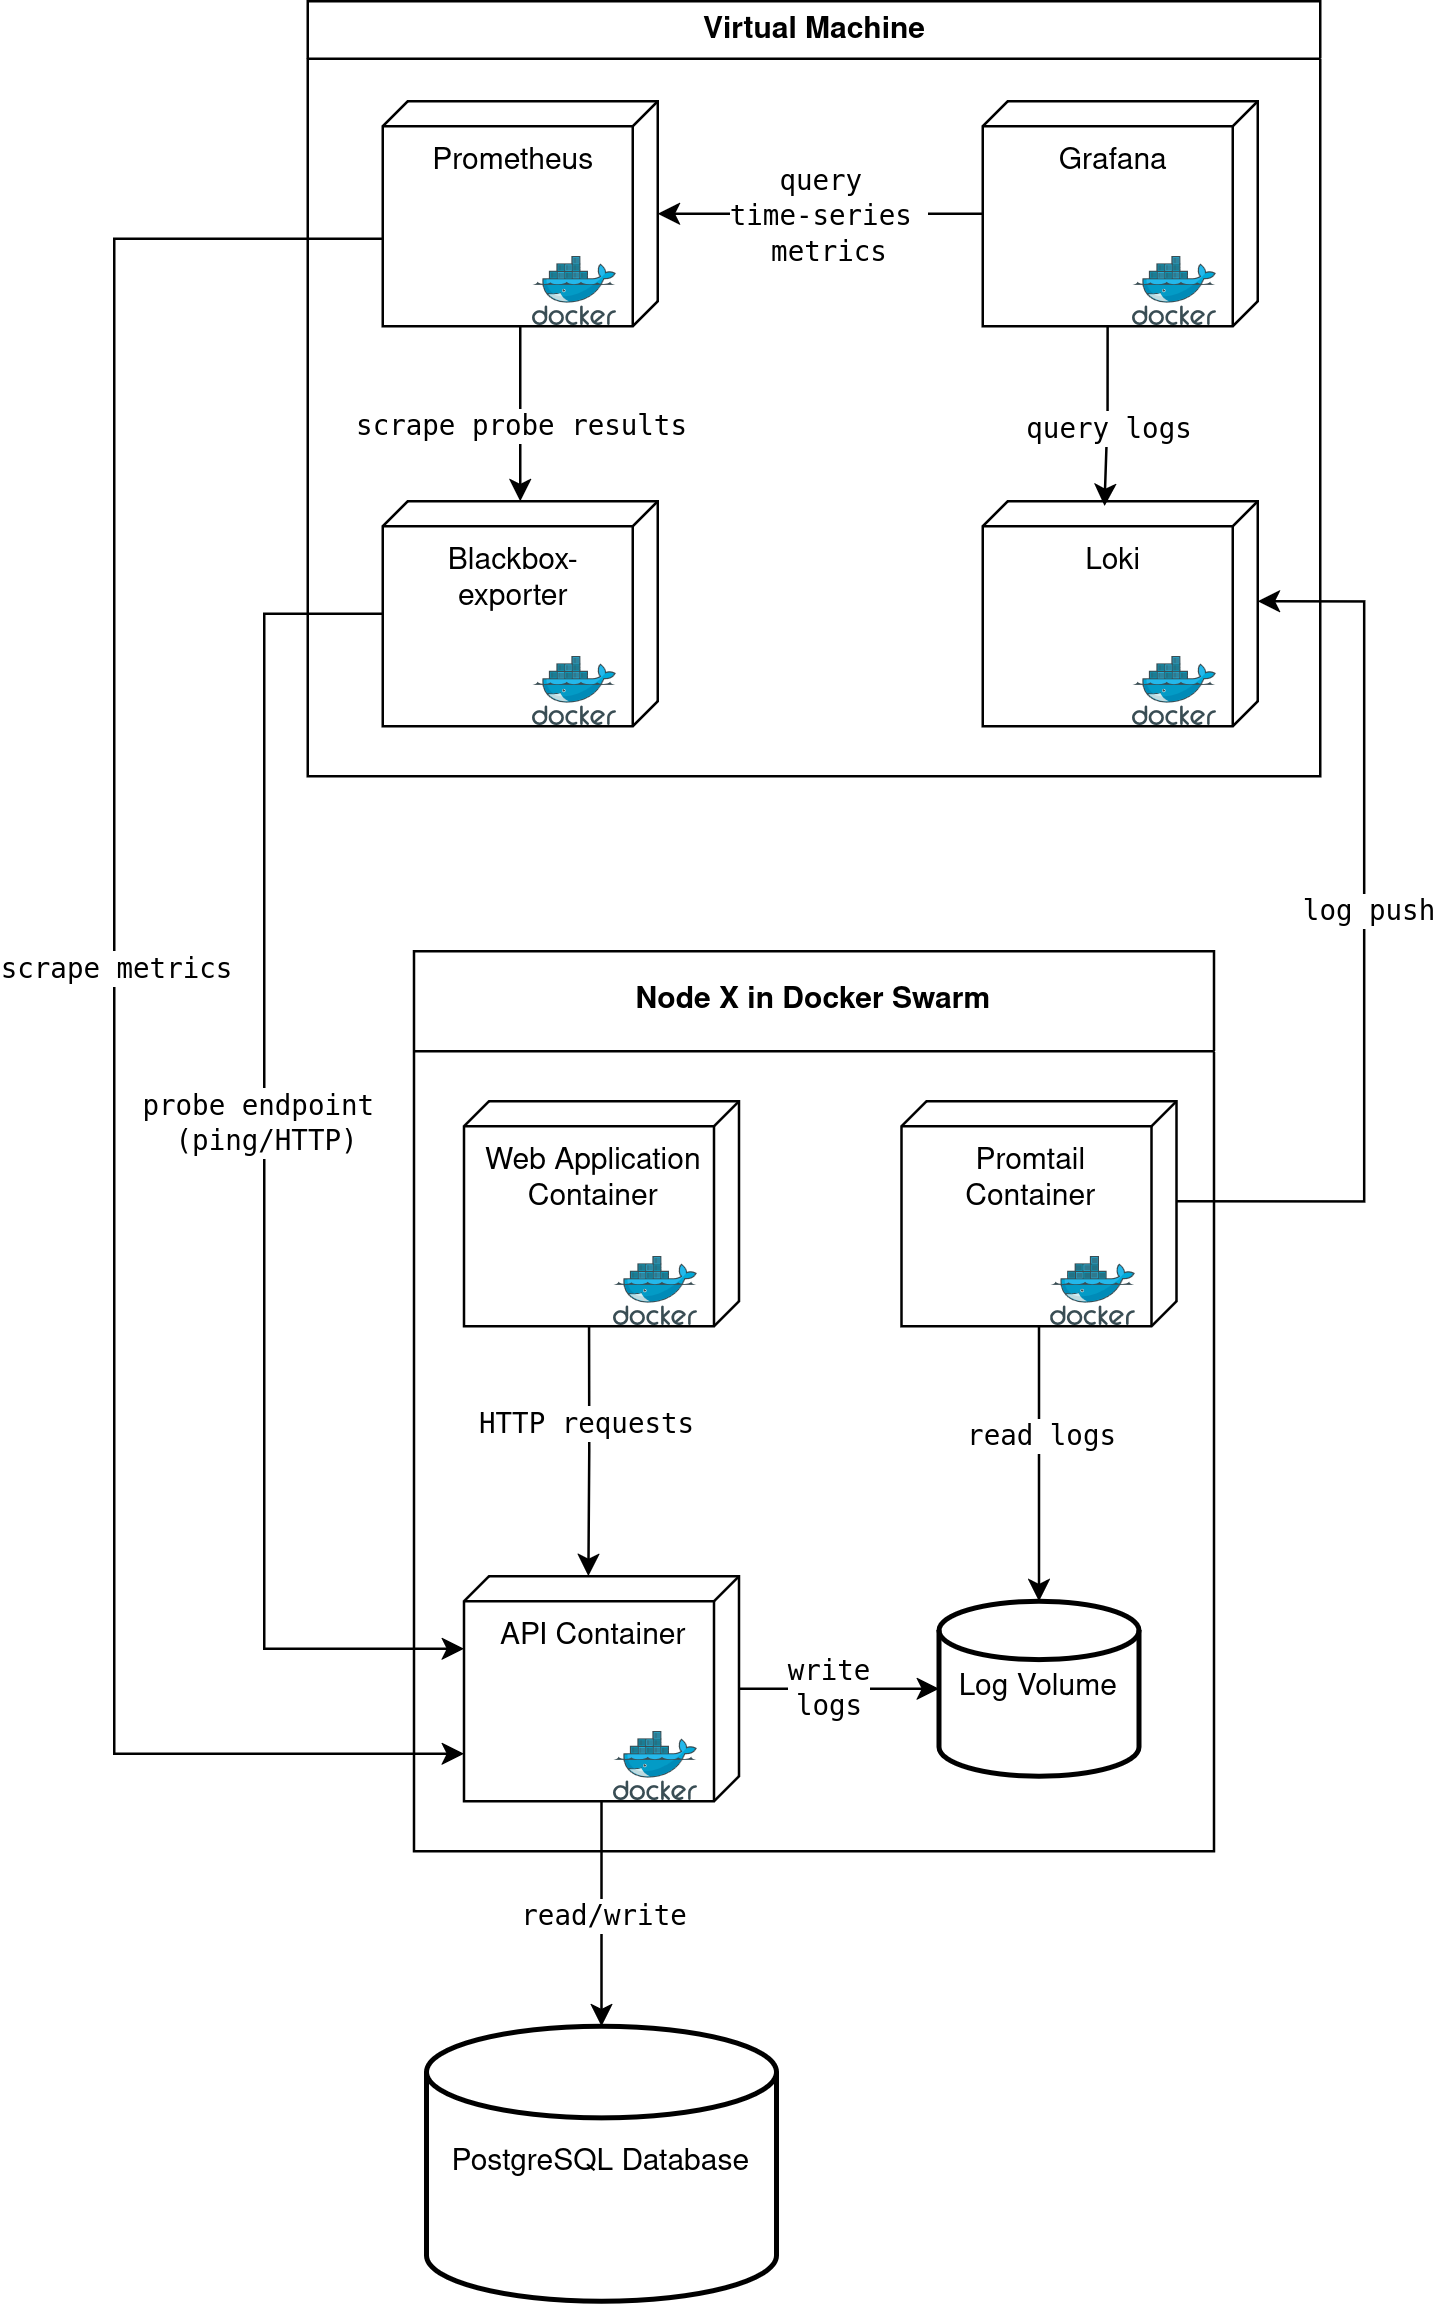
\includegraphics[width=0.4\textwidth]{report/images/monitoring-arch.png}
  \caption{Monitoring and Logging Architecture}
  \label{fig:monitoring-arch}
\end{figure}

For container orchestration and deployment, we used Docker Swarm to manage the distribution and scaling of our services across multiple nodes. Our Swarm cluster consists of one manager node and two worker nodes, each of which runs containers for the web application, API, and Promtail for log collection. Logs are written to a local log volume on each node and collected by Promtail, which forwards them to Loki for centralized aggregation.

This deployment model ensures both high availability and horizontal scalability, as containers are distributed and can be replicated across nodes. The architecture also separates concerns clearly—allowing us to manage application services independently from monitoring components. The diagram below illustrates the deployment structure across nodes in our cluster, highlighting the uniform setup of containers per node and the role of Promtail in the log pipeline.

\begin{figure}[H]
  \centering
  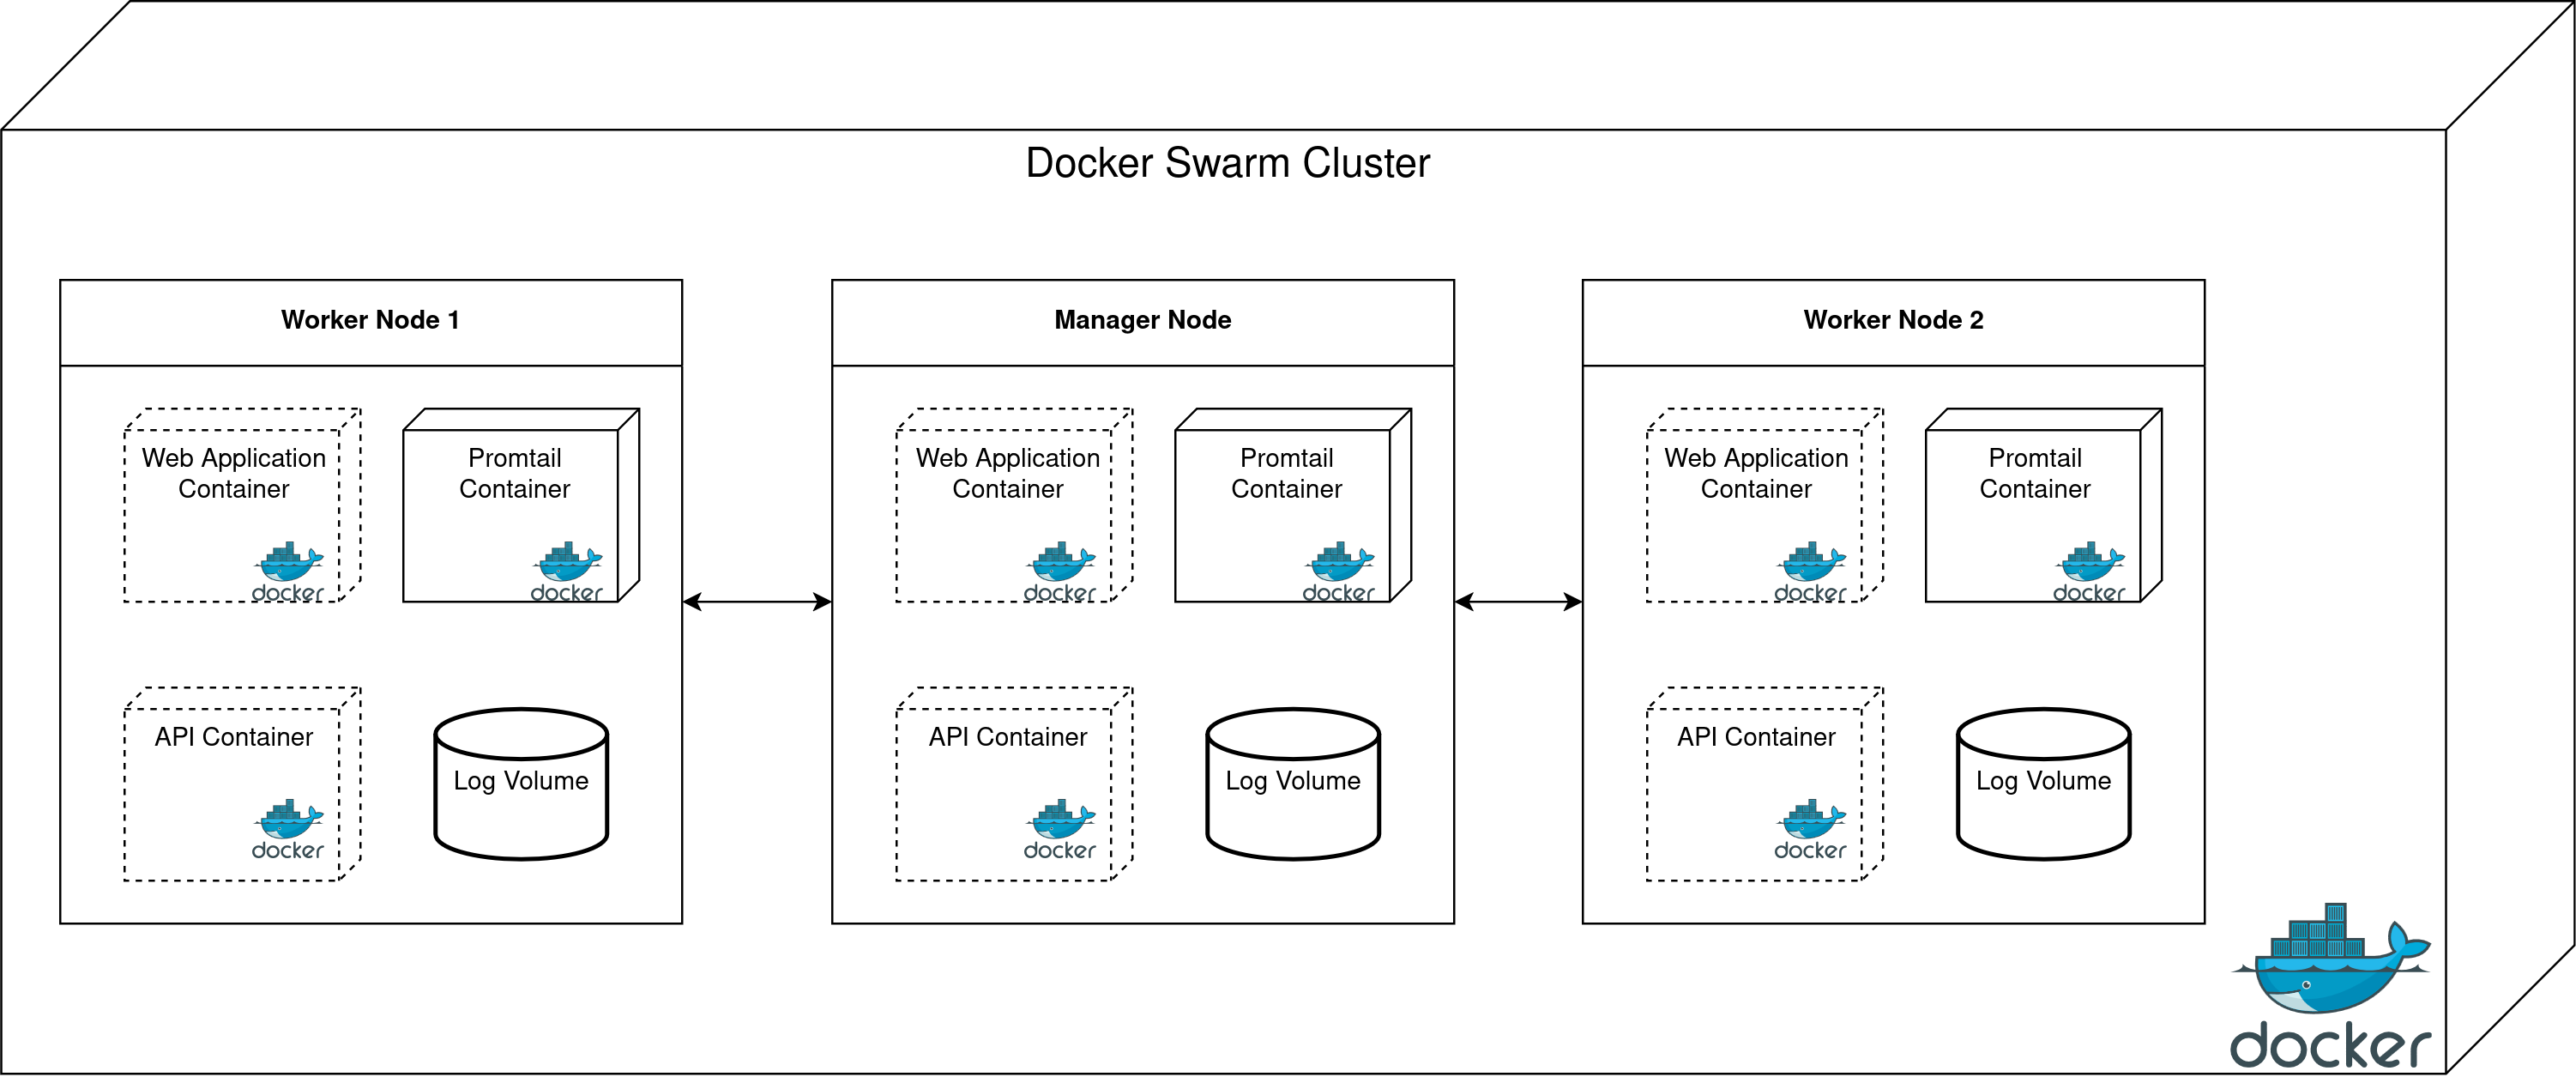
\includegraphics[width=0.6\textwidth]{report/images/docker-swarm.png}
  \caption{Deployment Diagram}
  \label{fig:docker-swarm}
\end{figure}


The Figure \ref{fig:arch-overview} shows the high level system architecture with a focus on request routing. We deployed the application using Docker Swarm across three virtual machines: one manager and two worker nodes as it shown in Figure \ref{fig:docker-swarm}. We used NGINX as a reverse proxy on the manager node to route HTTPS requests to the appropriate services.

All external traffic for our domain is first routed through Cloudflare, which handles HTTPS termination and DNS-based routing to the correct virtual machine. From there, NGINX forwards requests to the correct service ports inside the Docker Swarm. Services communicate securely, and our PostgreSQL database is accessed using TCP/IP with SSL to ensure encrypted communication.

This architecture ensures scalability, service isolation, and a clear separation of concerns.
\begin{figure}[H]
  \centering
  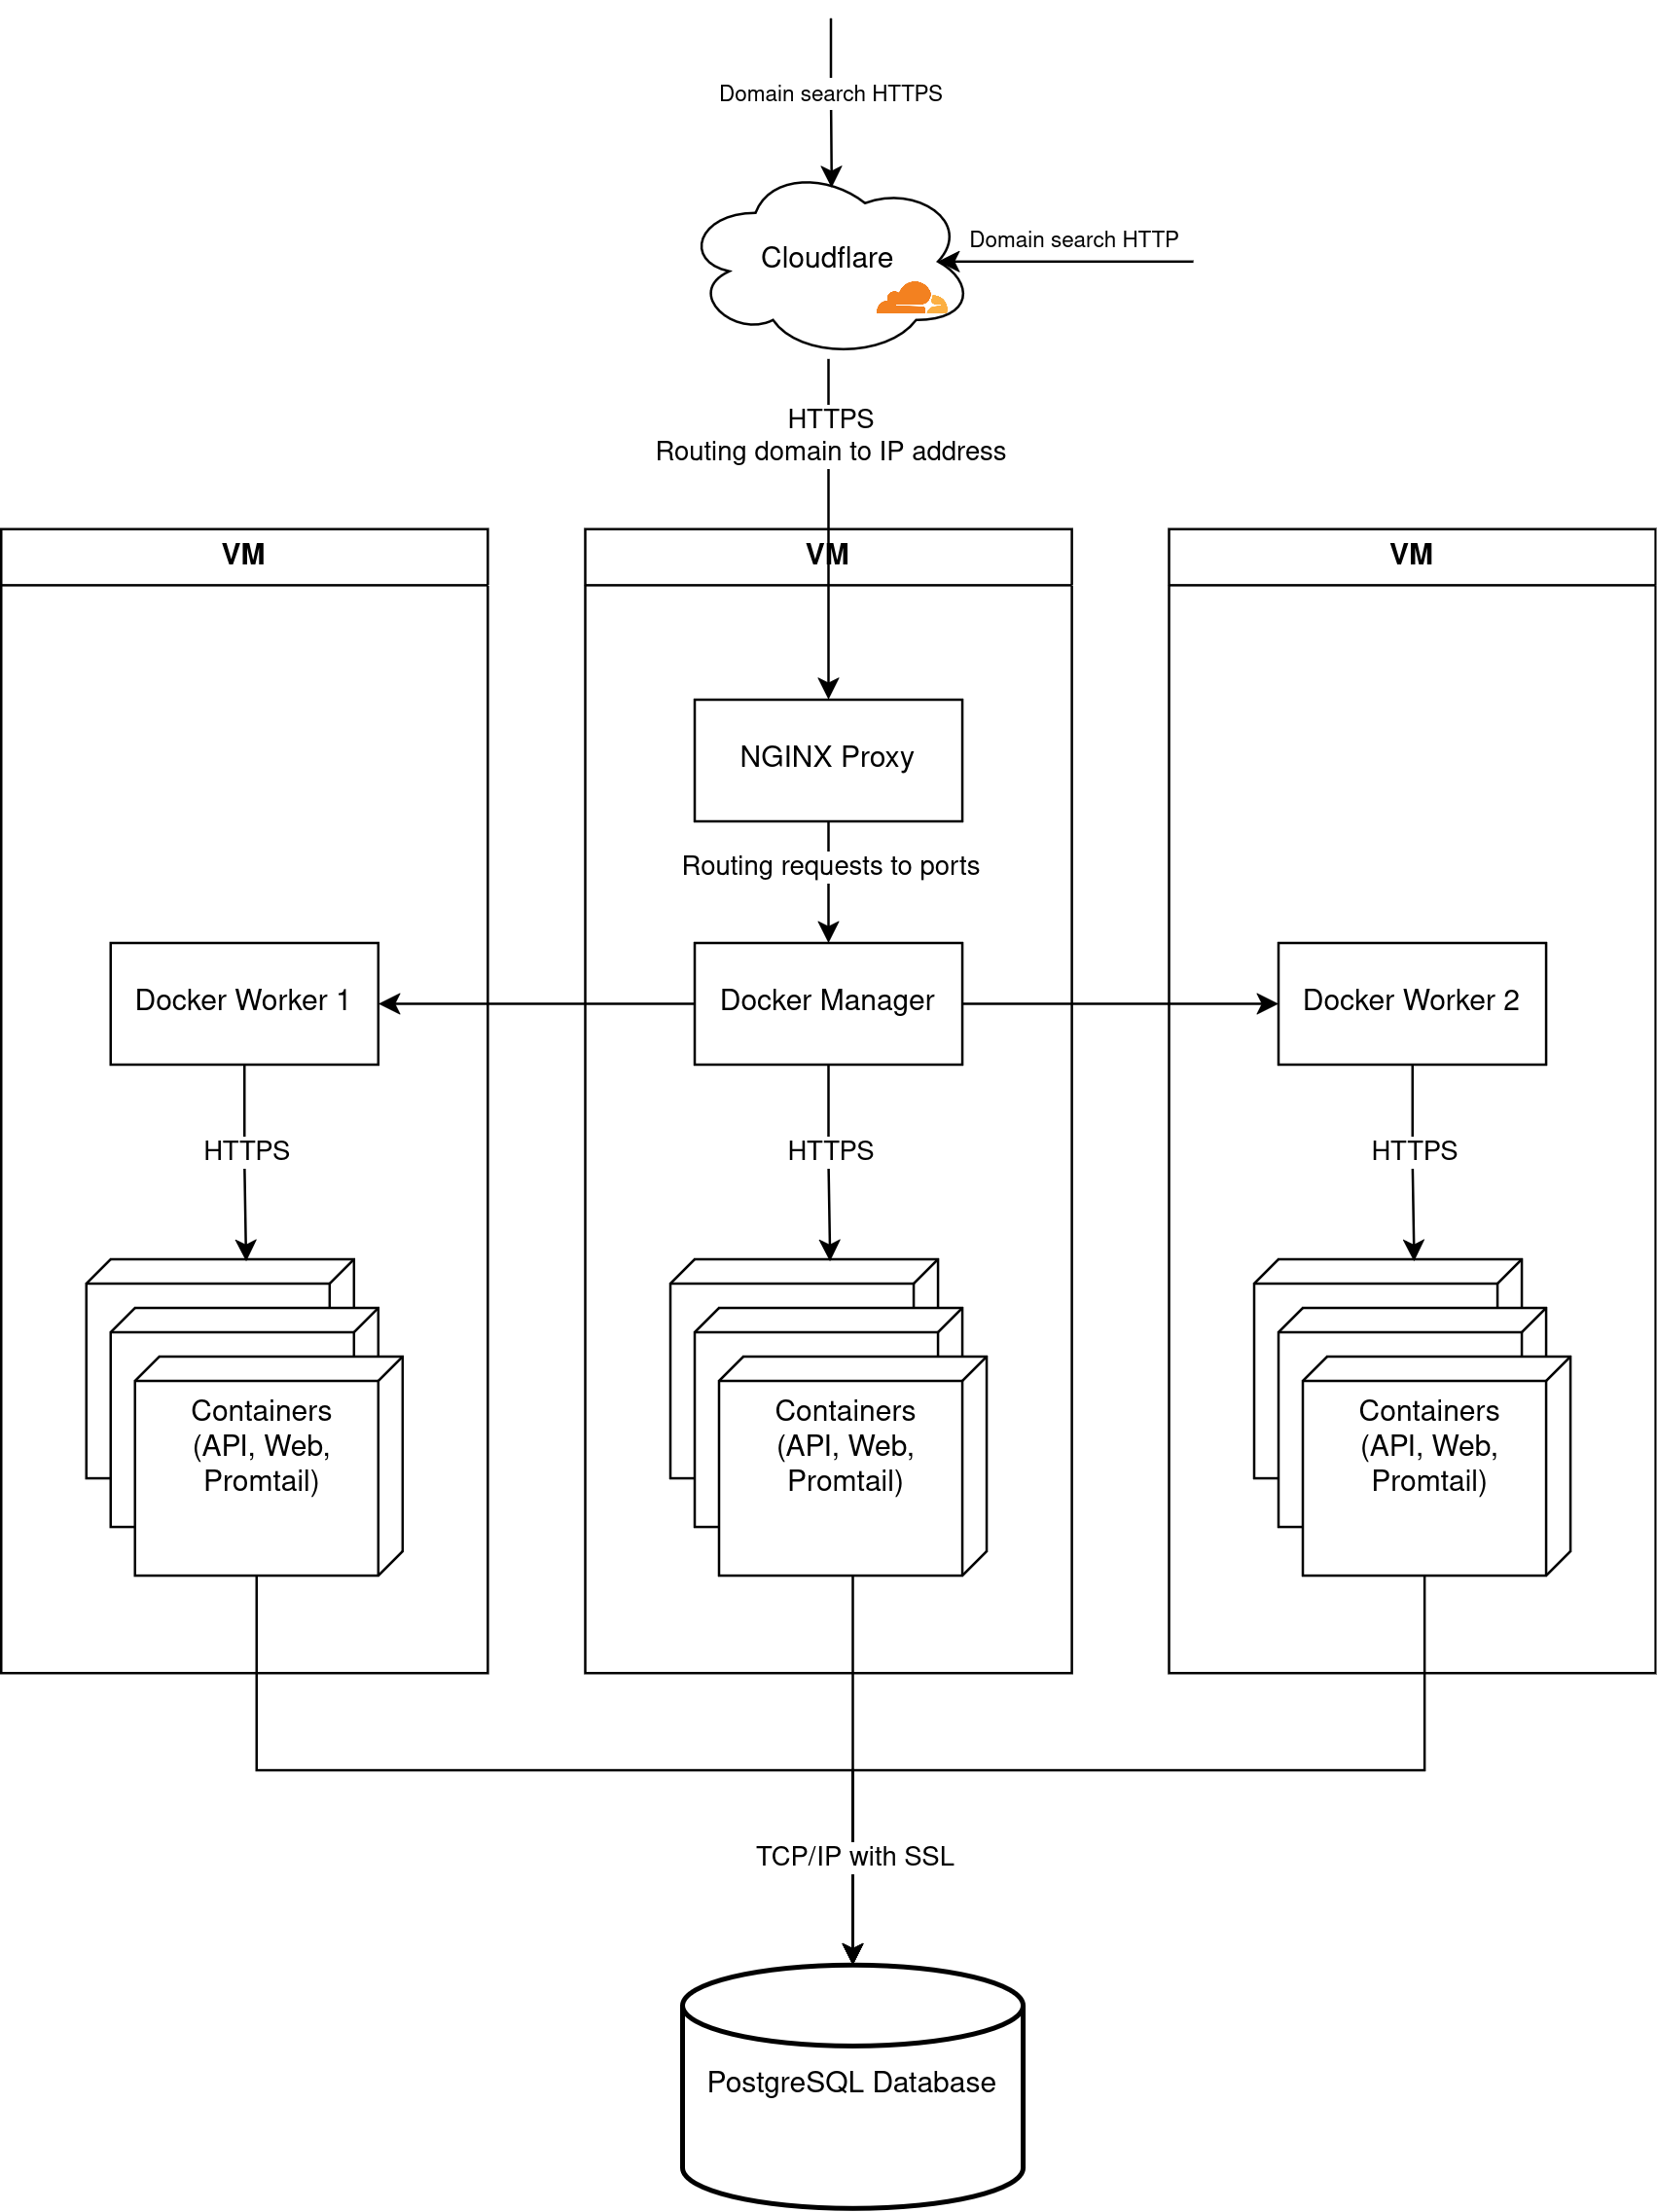
\includegraphics[width=0.4\textwidth]{report/images/arch-overview.png}
  \caption{System Architecture Overview}
  \label{fig:arch-overview}
\end{figure}


\subsection{Dependencies and Tooling}
\textbf{Frameworks}
\\
The application was refactored into Go to take advantage of its performance and built-in concurrency model. We mostly used Go’s standard library, which provides robust support for HTTP servers and routing out of the box. For more advanced routing, we incorporated the routing library \texttt{Gorilla Mux}\footnote{\url{https://github.com/gorilla/mux}}.
\\

\noindent \textbf{Containers and orchestration}
\\
We used Docker to containerize our application components, ensuring consistency across development, testing, and production environments. As the project evolved, we adopted Docker Swarm for container orchestration. This allowed us to manage multi-container deployments, scale services easily, and perform rolling updates with minimal downtime.
\\

\noindent \textbf{Database}
\\
When refactoring away from SQLite, we migrated to a PostgreSQL database which is managed and hosted by DigitalOcean. This provided better scalability, reliability, and support for multiple connections. We used the \texttt{GORM}\footnote{\url{https://gorm.io/}} library to introduce a Database abstraction layer so that we don't directly communicate with the database.
\\

\noindent \textbf{Others}
\\
We used a combination of Prometheus, Grafana, Loki, and Promtail. Prometheus was responsible for collecting metrics from our API. Grafana was used to visualize these metrics through their customizable dashboards. For centralized logging, we used Promtail to collect logs from our API and forward them to Loki, enabling us to query and visualize logs efficiently through Grafana’s interface.


\subsection{Subsystem Interactions}
%- Sequence diagram for user interaction flow 
\href{https://drive.google.com/file/d/18J39M3thQ0d2ehqQaVaydPF2SMUSb1fc/view?usp=sharing}{1st}
\begin{figure}[H]
  \centering
  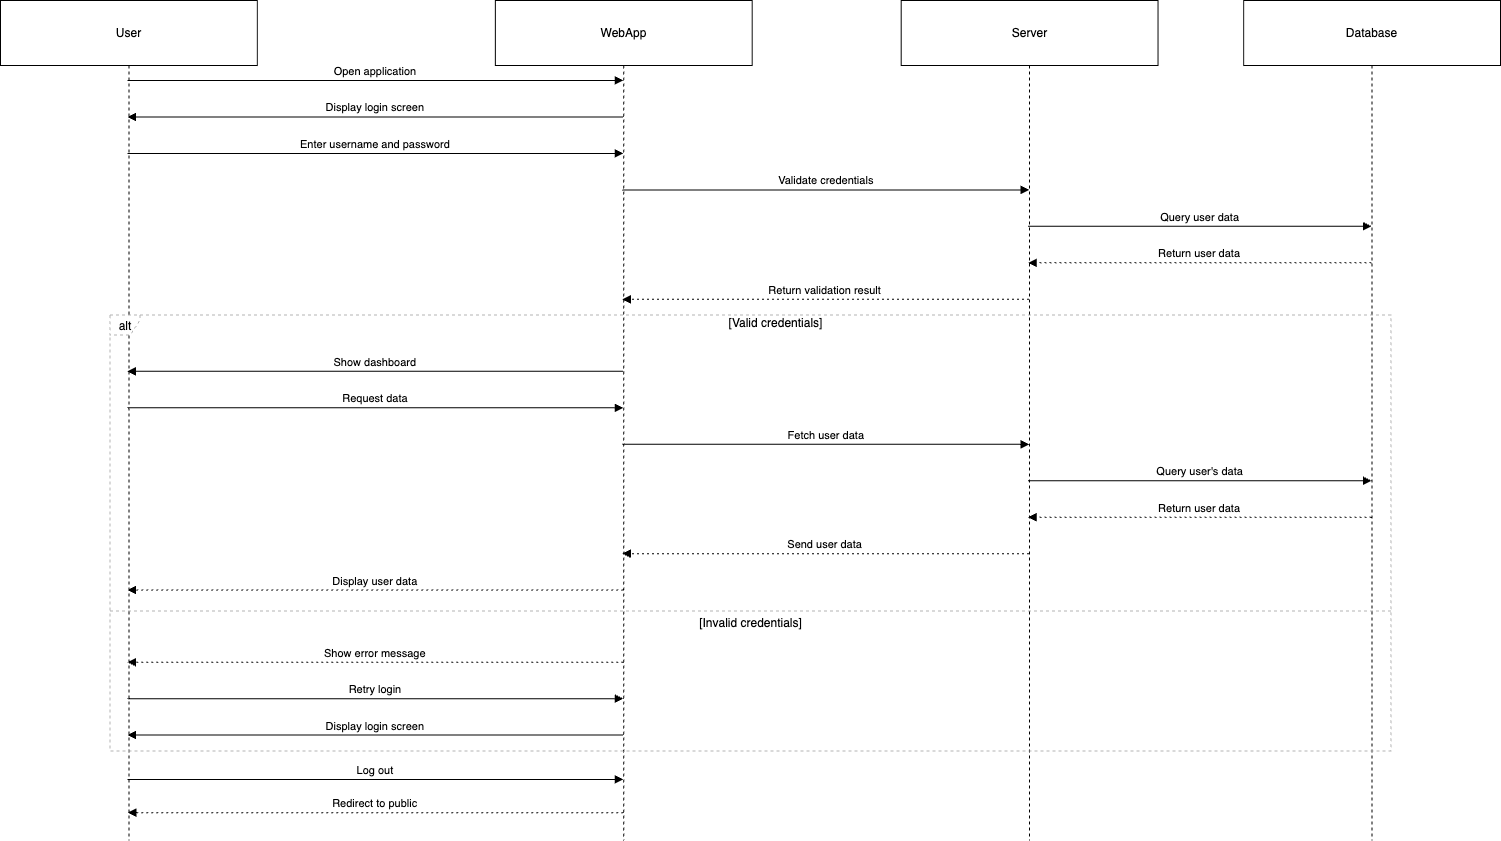
\includegraphics[width=\textwidth]{report/images/flow.png}
  \caption{Sequence diagram for user interaction flow }
  \label{fig:interaction}
\end{figure}
The flow and simulator diagrams only shows part of our System. There are other subsystem interactions, but we chose to stop here to not make the diagram too big. (Disclaimer: parts of the diagrams were created using the draw.io template prompt.)
\href{https://drive.google.com/file/d/1UtkS9Ijj9L4FBIYaqHKRZSK_WOFRrOoa/view?usp=sharing}{2nd}
\begin{figure}[H]
  \centering
  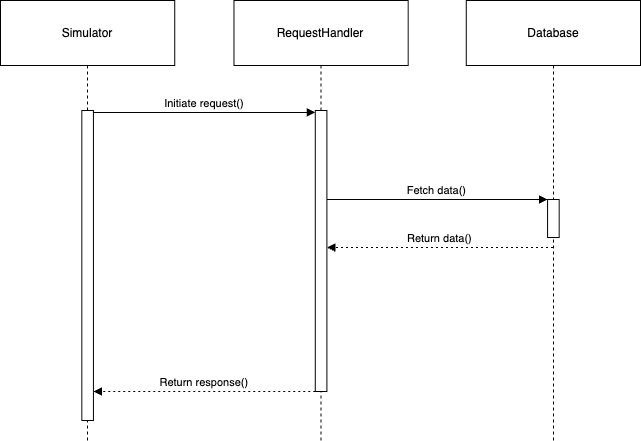
\includegraphics[width=\textwidth]{report/images/simulator.png}
  \caption{Sequence diagram for simulator}
  \label{fig:interaction}
\end{figure}


\subsection{Static Analysis and System Quality}
To ensure a maintainable and reliable system, we incorporated static analysis tools into our development workflow. These tools helped us improve code health and prevent technical debt accumulation.

We integrated three static analysis tools into our GitHub Actions CI/CD pipeline: \textbf{golangci-lint}, \textbf{Hadolint}, and \textbf{ShellCheck}. Each one of these tools targets a specific part of our codebase: Go code, Dockerfiles, and shell scripts respectively. The pipeline was configured in a dedicated workflow file, where each tool runs in a separate job.


For Go code, we used \textbf{golangci-lint} that runs multiple Go linters in parallel in a single configuration. This tool helped us uncover common issues such as unused imports or formatting violations. One notable finding involved detecting repeated logic and varaible declarations, especially in our test files. By refactoring the duplicated code into reusable functions, we improved both clarity and maintainability.

To ensure that our Dockerfiles follow the best practices we used \textbf{Hadolint}. This tools analyzes Dockerfiles for issues such as inefficient layers, missing CMD instructions or unsafe calls. To note is that Hadolint integrated ShellCheck internally, allowing it to lint shell commands embedded within Dockerfile RUN instructions.


While Hadolint covers shell code inside Dockerfiles, we used \textbf{ShellCheck} directly to lint external shell scripts in our repository. Integrating it in our pipeline ensured that all scripts were checked automatically before merging, catching quote issues and other unnecesarry subshells.

As a security measure, we integrated \textbf{GitGuardian}, a tool specifically designed to scan Git commits, branches, and CI pipelines for exposed secrets such as API keys, passwords, and other sensitive credentials. During testing, GitGuardian successfully identified an exposed a \textit{secret\_key} in one of our commits. Thanks to the immediate feedback from the pipeline, we were able to respond quickly by relocating the credentials to a dedicated \textit{.env} file, reducing the risk of leakage.

Lastly, we used \textbf{SonarQube} to gain insights into code quality metrics such as code duplication, complexity and any potential bugs. Unlike linters that enforce static rules, SonarQube focuses on maintainability and test coverage. One specific recommendation involved complex expressions muliple times in the same function, suggesting simplifying them to improve readability and testability.



\begin{comment}
\subsection{Design and architecture of your ITU-MiniTwit systems}
\subsection{All dependencies of your ITU-MiniTwit systems on all levels of abstraction and development stages. That is, list and briefly describe all technologies and tools you applied and depend on.}
\subsection{Important interactions of subsystems.}
\begin{itemize}
    \item For example, via an illustrative UML Sequence diagram that shows the flow of information through your system from user request in the browser, over all subsystems, hitting the database, and a response that is returned to the user. (gio)
    \item Similarly, another illustrative sequence diagram that shows how requests from the simulator traverse your system. (gio)
\end{itemize}
\subsection{Describe the current state of your systems, for example using results of static analysis and quality assessments.}
MSc students should argue for the choice of technologies and decisions for at least all cases for which we asked you to do so in the tasks at the end of each session.
\end{comment}